% ============================================================
% Beamer — ISLP Lecture Series — IMPROVED EDITION
% Advanced Module A11: Time Series and Forecasting
% ============================================================
\documentclass[aspectratio=169,11pt]{beamer}
\usepackage[utf8]{inputenc}\usepackage[T1]{fontenc}\usepackage[english]{babel}
\usepackage{graphicx}\usepackage{booktabs}\usepackage{amsmath,amssymb,amsfonts}
\usepackage{mathtools}\usepackage{hyperref}\usepackage{xcolor}
\usepackage{verbatim}\usepackage{alltt}
\usepackage{tikz}\usetikzlibrary{calc,arrows.meta,positioning,shapes}
\usepackage{tcolorbox}\tcbuselibrary{skins}

\usetheme{Madrid}\usecolortheme{default}
\setbeamertemplate{navigation symbols}{}
\setbeamertemplate{footline}[frame number]
\setbeamertemplate{blocks}[rounded][shadow=false]
\setbeamertemplate{headline}{%
  \leavevmode\hbox{%
    \begin{beamercolorbox}[wd=\paperwidth,ht=2.2ex,dp=0.9ex]{section in head/foot}%
      {\fontsize{4.6}{5.2}\selectfont%
       \insertsectionnavigationhorizontal{\paperwidth}{}{\hskip0pt plus1filll}}%
    \end{beamercolorbox}}%
}
\setbeamerfont{section in head/foot}{size=\tiny}
\setbeamerfont{palette primary}{size=\tiny}
\setbeamerfont{palette tertiary}{size=\tiny}
\setbeamerfont{section in toc}{size=\footnotesize}

\usepackage{listings}
\definecolor{pyKw}{RGB}{0,0,180}\definecolor{pyStr}{RGB}{20,120,40}
\definecolor{pyCom}{RGB}{120,120,120}\definecolor{accent}{RGB}{38,70,140}
\lstdefinestyle{Pystyle}{language=Python,basicstyle=\ttfamily\footnotesize,
  keywordstyle=\color{pyKw}\bfseries,commentstyle=\color{pyCom}\itshape,
  stringstyle=\color{pyStr},showstringspaces=false,upquote=true,
  columns=fullflexible,breaklines=true,literate={~}{{$\sim$}}1}
\lstset{style=Pystyle}

% Tighter TOC spacing (place AFTER \lstset, BEFORE \AtBeginSection)
\usepackage{etoolbox}
\makeatletter
\patchcmd{\beamer@sectionintoc}{\vskip1.5em}{\vskip.6em}{\typeout{TOCPATCH-OK}}{\typeout{TOCPATCH-FAIL}}
\makeatother

\AtBeginSection[]{\begin{frame}{Outline}\footnotesize
  \tableofcontents[currentsection,sectionstyle=show/shaded,subsectionstyle=show/show/hide]
\end{frame}}

\newcommand{\islpsource}[1]{%
  \vfill\hfill{\tiny\itshape\color{gray}Source: #1 \textemdash{} ISLP, James et al.\ (2023).}\par
}

\newtcolorbox{takeaway}[1][Takeaway]{enhanced,colback=green!4,colframe=green!50!black,
  boxrule=0pt,leftrule=2.5pt,arc=2pt,fonttitle=\bfseries,title=#1,
  left=2mm,right=2mm,top=1mm,bottom=1mm}
\newtcolorbox{numexample}[1][Worked example]{enhanced,colback=orange!4,colframe=orange!70!black,
  boxrule=0pt,leftrule=2.5pt,arc=2pt,fonttitle=\bfseries,title=#1,
  left=2mm,right=2mm,top=1mm,bottom=1mm}
\newtcolorbox{readme}[1][How to read this]{enhanced,colback=blue!4,colframe=accent,
  boxrule=0pt,leftrule=2.5pt,arc=2pt,fonttitle=\bfseries,title=#1,
  left=2mm,right=2mm,top=1mm,bottom=1mm}

\title{Quantitative Research Methods}
\subtitle{Time Series and Forecasting\\[2pt]{\small Advanced module A11 --- optional self-study}}
\author{Prof.\ Dr.\ Christoph Weisser}
\date{}\graphicspath{{images/}}

\newtcolorbox{exercise}[1][Exercise]{enhanced, fontupper=\footnotesize, colback=purple!4, colframe=purple!55!black, boxrule=0pt, leftrule=2.5pt, arc=2pt, fonttitle=\bfseries, title=#1, left=2mm, right=2mm, top=1mm, bottom=1mm}
\newtcolorbox{solutionbox}[1][Solution]{enhanced, colback=teal!5, colframe=teal!55!black, boxrule=0pt, leftrule=2.5pt, arc=2pt, fonttitle=\bfseries, title=#1, left=2mm, right=2mm, top=1mm, bottom=1mm}
\newtcolorbox{longexercise}[1][Extended exercise (15 min)]{enhanced, fontupper=\footnotesize, colback=violet!6, colframe=violet!55!black, boxrule=0pt, leftrule=3pt, arc=2pt, fonttitle=\bfseries, title=#1, left=2mm, right=2mm, top=1mm, bottom=1mm}

% Reclaim ~2pt of body height (custom nav headline makes full slides tip over by ~1.83pt)
\addtobeamertemplate{frametitle}{}{\vspace{-2pt}}

\newtcolorbox{labnote}[1][Run this live in the lab notebook]{enhanced, fontupper=\footnotesize, colback=cyan!7, colframe=cyan!45!black, boxrule=0pt, leftrule=3pt, arc=2pt, fonttitle=\bfseries, title=#1, left=2mm, right=2mm, top=1mm, bottom=1mm}

% Common-mistake callout --- crimson, for the error to pre-empt
\newtcolorbox{mistake}[1][Common mistake]{enhanced, fontupper=\footnotesize, colback=red!4, colframe=red!60!black, boxrule=0pt, leftrule=3pt, arc=2pt, fonttitle=\bfseries, title=#1, left=2mm, right=2mm, top=1mm, bottom=1mm}

\begin{document}
\begin{frame}[plain]\titlepage\end{frame}

\begin{frame}{Where this module fits}
  \footnotesize
  \begin{center}
  \begin{tabular}{@{}p{3.9cm}p{8.4cm}@{}}
    \toprule
    \textbf{Course chapter / module} & \textbf{What this module builds on it} \\
    \midrule
    Ch.\ 3 --- linear regression & AR models \emph{are} least squares on lagged copies \\
    Ch.\ 4 --- classification & \texttt{Weekly}/\texttt{Smarket}: time-ordered data we treated as rows \\
    Ch.\ 5 --- resampling & The one pitfall Ch.\ 5 names but never resolves: CV on time \\
    Ch.\ 7 --- beyond linearity & Seasonal profiles are Chapter 7 curves in disguise \\
    \bottomrule
  \end{tabular}
  \end{center}
  \vspace{2pt}
  \begin{takeaway}[The row that knows its neighbours]
    Every taught chapter shuffles rows freely, because rows are independent. A time
    series is the opposite: \textbf{the order is the information}. This module makes
    the order visible (autocorrelation), models it (AR), and evaluates honestly
    (backtesting).
  \end{takeaway}
  {\scriptsize One of twelve optional advanced modules; self-study. Every number on
  these slides is reproduced by \texttt{make\_figures.py} in the module folder.}
\end{frame}

\begin{frame}{Contents}\small\tableofcontents[hideallsubsections]
  \vfill
  {\tiny Optional and advanced material is collected in the \textbf{appendix} at the end of the deck.}
\end{frame}

\begin{frame}{Notation in this module}
  \footnotesize
  \begin{center}
  \begin{tabular}{@{}ll@{}}
    \toprule
    \textbf{Symbol} & \textbf{Meaning} \\
    \midrule
    $y_t$ & the observation at time $t$; order matters \\
    $y_{t-k}$ & the $k$-th \emph{lag} of the series \\
    $r_k$ & sample autocorrelation at lag $k$ (the ACF) \\
    $\phi$ & AR coefficient(s) \\
    AR($p$) & regression of $y_t$ on its own last $p$ values \\
    $\hat y_{T+h\mid T}$ & forecast of horizon $h$ made with data up to $T$ \\
    $\varepsilon_t$ & white noise: mean $0$, no autocorrelation \\
    MAE & mean absolute error of a forecast \\
    \bottomrule
  \end{tabular}
  \end{center}
\end{frame}

\begin{frame}{Sources and references}
  \begin{block}{Primary textbook}
    James, Witten, Hastie, Tibshirani \& Taylor (2023),
    \emph{An Introduction to Statistical Learning, with Applications in Python},
    Springer. --- \texttt{Bikeshare} and \texttt{Weekly} are its bundled datasets;
    ISLP \S 10.5 sketches sequences, this module develops them.
  \end{block}
  \begin{block}{Canonical further reading (optional)}
    Hyndman \& Athanasopoulos, \emph{Forecasting: Principles and Practice} (3rd ed.,
    online) --- the standard applied reference; everything here scales up there.
  \end{block}
\end{frame}

\begin{frame}{Learning objectives}
  By the end of this module you will be able to:
  \begin{itemize}
    \item \textbf{Explain} why i.i.d.\ reasoning fails on ordered data, and what
          replaces it (stationarity, autocorrelation).
    \item \textbf{Compute} and read an ACF --- by hand on six numbers, and in code
          on $8{,}645$.
    \item \textbf{Fit} an AR model as a Chapter 3 regression on lagged copies, and
          state when it is stationary.
    \item \textbf{Beat} the two baselines every forecast must beat: the global mean
          and the seasonal naive.
    \item \textbf{Evaluate} honestly with a rolling-origin backtest --- and say
          precisely what shuffled cross-validation gets wrong.
  \end{itemize}
\end{frame}

\begin{frame}{Roadmap of this module}
  \begin{takeaway}[From plotted order to honest forecasts]
    \begin{enumerate}
      \item The problem: rows that remember --- and Chapter 5's unanswered question.
      \item Seeing structure: the series, its seasonal profiles, the ACF.
      \item AR models: least squares on the past, stationarity, baselines.
      \item Honest evaluation: rolling-origin backtests vs shuffled CV.
      \item A financial postscript: why returns resist all of this.
      \item Python lab, summary, appendix.
    \end{enumerate}
  \end{takeaway}
\end{frame}

% ============================================================
\section{The Problem}
% ============================================================

\begin{frame}{One year of hourly bike rentals}
  \begin{center}
    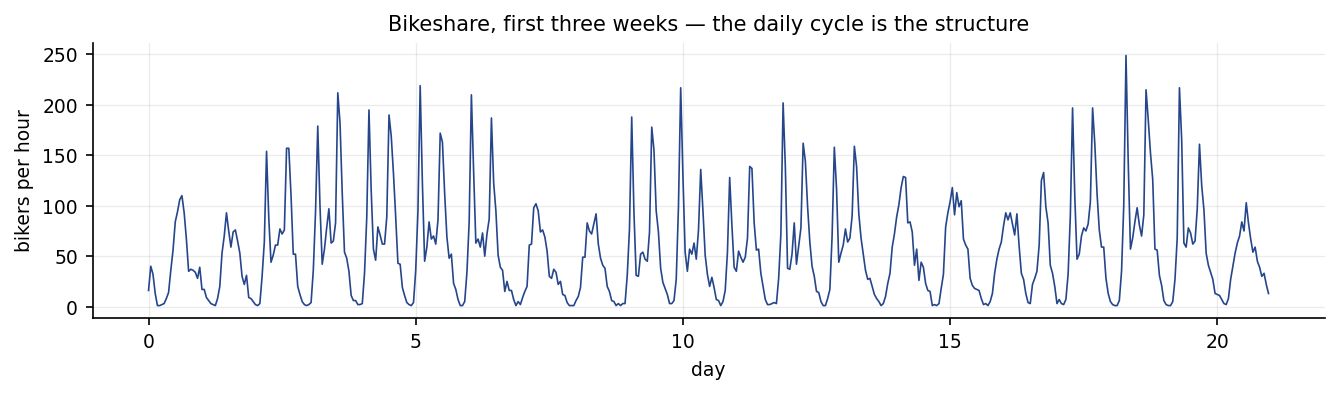
\includegraphics[width=0.94\textwidth,height=0.44\textheight,keepaspectratio]{cha11_series.png}
  \end{center}
  \begin{takeaway}[The order is the signal]
    \texttt{Bikeshare}: $8{,}645$ hourly counts, mean $144$, max $651$. Chapter 4 met
    this dataset as exchangeable rows; plotted \emph{in order} it is almost
    periodic. Shuffle the rows and this structure --- most of the predictability ---
    is destroyed.
  \end{takeaway}
\end{frame}

\begin{frame}{What independence buys you --- and what its loss costs}
  \begin{center}
  \footnotesize
  \begin{tabular}{@{}lll@{}}
    \toprule
    & \textbf{i.i.d.\ rows (Ch.\ 1--8)} & \textbf{time series} \\
    \midrule
    information per row & full & partly shared with neighbours \\
    train/test split & any random split & \emph{past} trains, \emph{future} tests \\
    CV (Ch.\ 5) & shuffle freely & shuffling leaks the future \\
    the mean & the natural predictor & often the \emph{worst} sane predictor \\
    new data & more of the same & possibly a different regime \\
    \bottomrule
  \end{tabular}
  \end{center}
  \begin{readme}[The one new assumption]
    \footnotesize
    In place of independence we assume \textbf{stationarity}: the joint distribution
    of $(y_t, y_{t+k})$ does not depend on $t$ --- levels, spreads and correlations
    are stable over time. It plays the role exchangeability played in module A3:
    the licence for learning from the past at all.
  \end{readme}
\end{frame}

\begin{frame}{Exercise A11.1 --- Where does the leak happen? [Concept]}
  \begin{exercise}
    A colleague fits a model to three years of daily sales, evaluates it with
    shuffled 10-fold CV from Chapter 5, reports MAE $= 41$, deploys --- and
    measures MAE $= 70$ in production.
    \begin{enumerate}
      \item Explain the mechanism of the failure in two sentences: what exactly did
            the shuffled folds let the model see?
      \item Their model uses only \emph{calendar features} (weekday, month) --- no
            lags. Does the argument change?
      \item Propose the evaluation they should have run.
    \end{enumerate}
  \end{exercise}
\end{frame}

\begin{frame}{Solution --- Exercise A11.1}
  \begin{solutionbox}
    \footnotesize
    \textbf{Part 1.} In a shuffled fold, the days immediately before and after each
    test day sit in the training set. Sales on neighbouring days are strongly
    correlated, so the model effectively \emph{interpolates between known
    neighbours} --- a much easier task than the production task, which is
    \emph{extrapolating beyond the last known day}. The CV number answers the wrong
    question.
    \par\smallskip
    \textbf{Part 2.} It softens but does not vanish. With purely calendar features
    the model cannot copy neighbours directly --- but the folds still share the
    \emph{level} of each local stretch (this year's demand regime), so drifting
    levels and new regimes are still invisible to shuffled CV. The gap of
    $41 \to 70$ typically has both components.
    \par\smallskip
    \textbf{Part 3.} A \textbf{rolling-origin backtest}: train on data up to time
    $T$, forecast the next horizon, roll $T$ forward, repeat; report the average
    error over origins. It rehearses deployment exactly.
  \end{solutionbox}
  \begin{mistake}
    ``We used cross-validation, so the estimate is honest.'' Chapter 5's guarantee
    rests on exchangeable rows; time-ordered rows are the textbook case where it
    breaks.
  \end{mistake}
\end{frame}

% ============================================================
\section{Seeing Structure}
% ============================================================

\begin{frame}{Two clocks: the day and the year}
  \begin{center}
    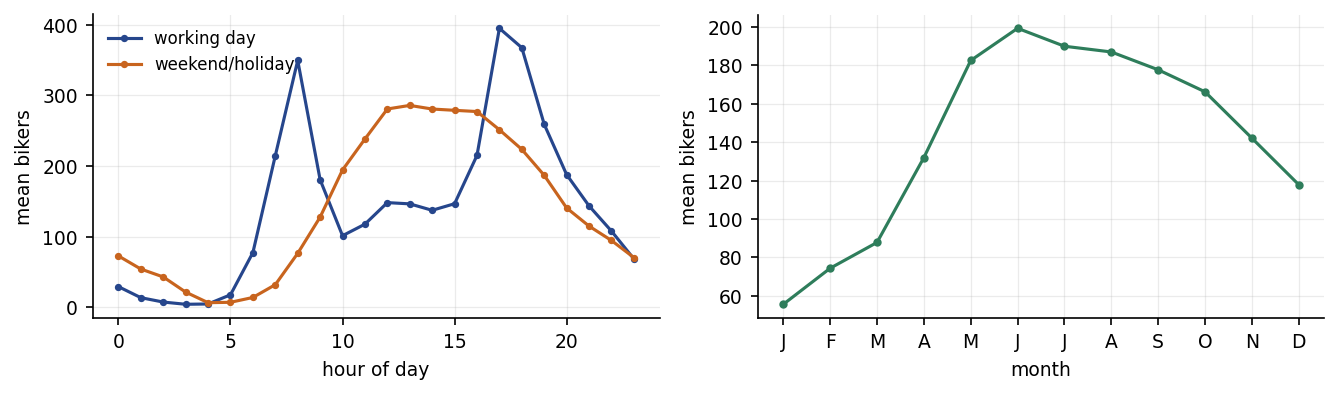
\includegraphics[width=0.94\textwidth,height=0.42\textheight,keepaspectratio]{cha11_profiles.png}
  \end{center}
  \begin{takeaway}[Seasonality is just a curve over a clock]
    Working days peak at \textbf{hour 17} with a morning twin at 8 --- commuting.
    Weekends have one broad afternoon hump. Months carry a second, annual cycle.
    Each profile is a Chapter 7 curve fitted over a circular clock --- nothing
    beyond the taught course.
  \end{takeaway}
\end{frame}

\begin{frame}{The autocorrelation function: correlation with your own past}
  \begin{block}{Rule}
    \[
      \boxed{\; r_k = \frac{\sum_{t=k+1}^{T} (y_t - \bar y)(y_{t-k} - \bar y)}
      {\sum_{t=1}^{T} (y_t - \bar y)^2} \;}
      \qquad k = 1, 2, \dots
    \]
  \end{block}
  \begin{readme}[How to read this]
    \footnotesize
    It is Chapter 3's correlation coefficient, computed between the series and a
    $k$-shifted copy of itself (one shared normaliser). $r_k \approx 0$ at all lags
    $\Rightarrow$ white noise, nothing to forecast. For pure noise,
    $|r_k| < 1.96/\sqrt{T}$ about $95\%$ of the time --- the dotted band on every
    ACF plot ($\pm 0.021$ here).
  \end{readme}
  \begin{numexample}[Bikeshare's memory]
    $r_1 = \mathbf{0.84}$: this hour looks like last hour. $r_{24} = \mathbf{0.79}$:
    this hour looks like the same hour yesterday. Both dwarf the noise band ---
    two separate memories, and an AR model should be offered \emph{both}.
  \end{numexample}
\end{frame}

\begin{frame}{The ACF, drawn}
  \begin{center}
    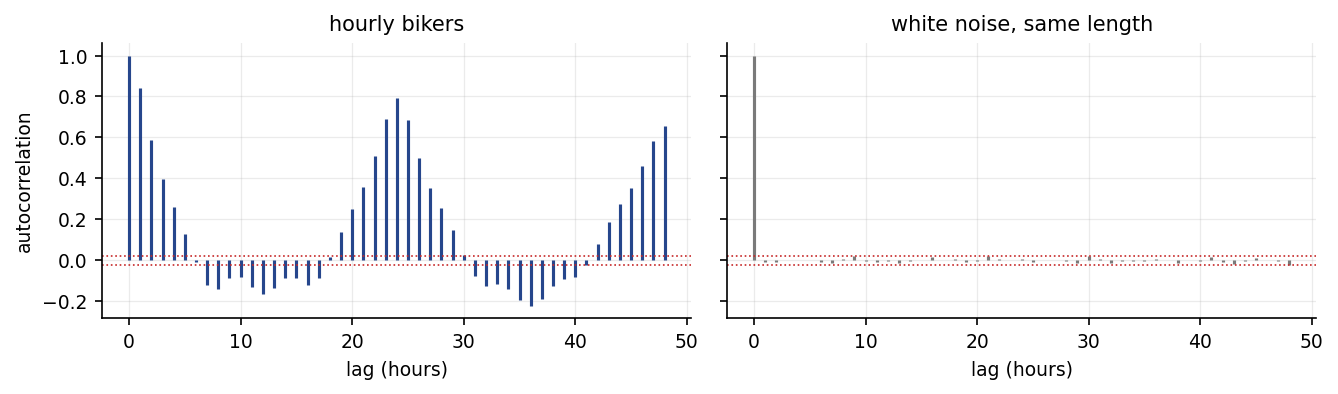
\includegraphics[width=0.94\textwidth,height=0.44\textheight,keepaspectratio]{cha11_acf.png}
  \end{center}
  \begin{takeaway}[Structure vs nothing]
    Left: bikers --- slow decay from $r_1 = 0.84$ plus a clean spike ridge at lag
    $24$ and its multiples. Right: white noise of the same length --- everything
    inside $\pm 0.021$. The ACF is the module's diagnostic instrument: it tells you
    \emph{whether} and \emph{where} the past is informative.
  \end{takeaway}
\end{frame}

\begin{frame}{The same fact as a scatter plot}
  \begin{center}
    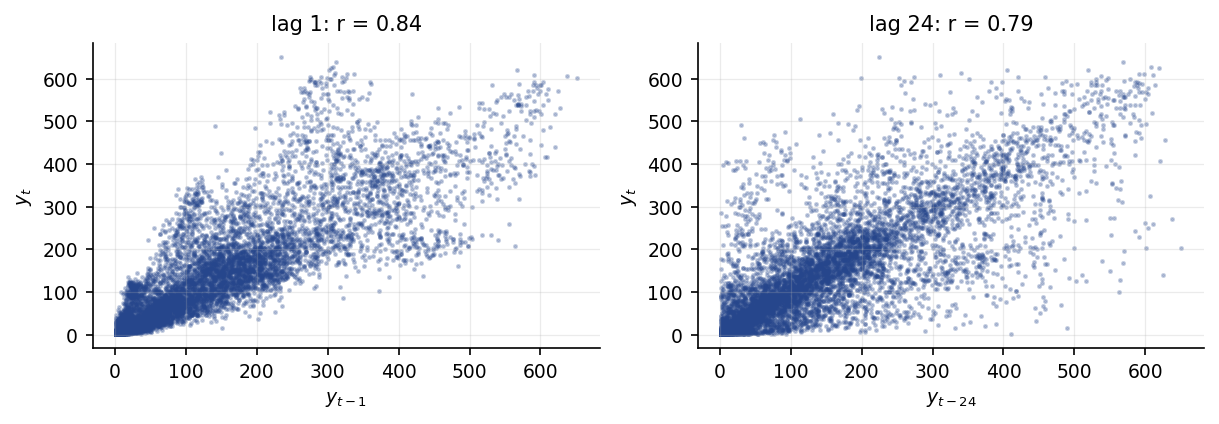
\includegraphics[width=0.82\textwidth,height=0.46\textheight,keepaspectratio]{cha11_lagscatter.png}
  \end{center}
  \begin{takeaway}[Lag plots are Chapter 2 pictures]
    Plot $y_t$ against $y_{t-1}$ ($r = 0.84$) or against $y_{t-24}$ ($r = 0.79$)
    and forecasting collapses into the course's oldest picture: a supervised
    scatter with a strong linear signal --- the predictors just happen to be the
    outcome's own past.
  \end{takeaway}
\end{frame}

\begin{frame}{Exercise A11.2 --- An ACF by hand [Math]}
  \begin{exercise}
    A tiny series: $y = (3,\; 5,\; 4,\; 6,\; 5,\; 7)$.
    \begin{enumerate}
      \item Compute $\bar y$ and the deviations.
      \item Compute $r_1$ and $r_2$ from the formula (shared denominator).
      \item One of the two is negative and one clearly positive. Describe the
            pattern in the data that produces exactly this pair.
    \end{enumerate}
  \end{exercise}
\end{frame}

\begin{frame}{Solution --- Exercise A11.2}
  \begin{solutionbox}
    \footnotesize
    \textbf{Part 1.} $\bar y = 30/6 = 5$; deviations $d = (-2, 0, -1, 1, 0, 2)$.
    \par\smallskip
    \textbf{Part 2.} Denominator $\sum d_t^2 = 4 + 0 + 1 + 1 + 0 + 4 = 10$.
    \[
      r_1 = \tfrac{(-2)(0) + (0)(-1) + (-1)(1) + (1)(0) + (0)(2)}{10}
          = \tfrac{-1}{10} = \mathbf{-0.1},
    \]
    \[
      r_2 = \tfrac{(-2)(-1) + (0)(1) + (-1)(0) + (1)(2)}{10}
          = \tfrac{4}{10} = \mathbf{+0.4}.
    \]
    \textbf{Part 3.} The series zig-zags: each value overshoots then undershoots a
    rising path --- so adjacent values are (mildly) anti-correlated, while values
    two apart sit on the same side of the zig-zag and agree. A period-2
    alternation shows up as exactly this sign pattern, the miniature of
    Bikeshare's period-24 ridge.
  \end{solutionbox}
  \begin{mistake}
    Recomputing the denominator on the shortened overlap for each lag. The standard
    ACF divides every lag by the \emph{same} full-series sum of squares --- that is
    what makes $r_k$ comparable across $k$.
  \end{mistake}
\end{frame}

% ============================================================
\section{AR Models}
% ============================================================

\begin{frame}{The autoregression: Chapter 3 pointed at the past}
  \begin{block}{Rule}
    \[
      \text{AR}(p): \quad
      \boxed{\; y_t = \beta_0 + \phi_1 y_{t-1} + \phi_2 y_{t-2} + \cdots
        + \phi_p y_{t-p} + \varepsilon_t \;}
    \]
    Build the lagged copies as columns, then fit by \textbf{ordinary least squares}.
  \end{block}
  \begin{readme}[How to read this]
    \footnotesize
    There is no new estimator here: make a design matrix whose columns are
    $y_{t-1}, y_{t-2}, \dots$ and run Chapter 3. The art moves into
    \emph{which lags to offer}: the ACF said Bikeshare has an hourly memory
    \textbf{and} a daily one, so we offer lags $1, 2$ (recent hours), $24, 25$
    (yesterday) and $168$ (last week).
  \end{readme}
  \begin{numexample}[The fitted coefficients]
    On lags $(1, 2, 24, 25, 168)$:
    $\hat\phi = (0.83,\, -0.20,\, 0.51,\, -0.38,\, 0.18)$ --- last hour dominates,
    yesterday's same hour adds half a weight, last week a little more.
  \end{numexample}
\end{frame}

\begin{frame}{Stationarity: when does an AR(1) settle down?}
  \begin{center}
    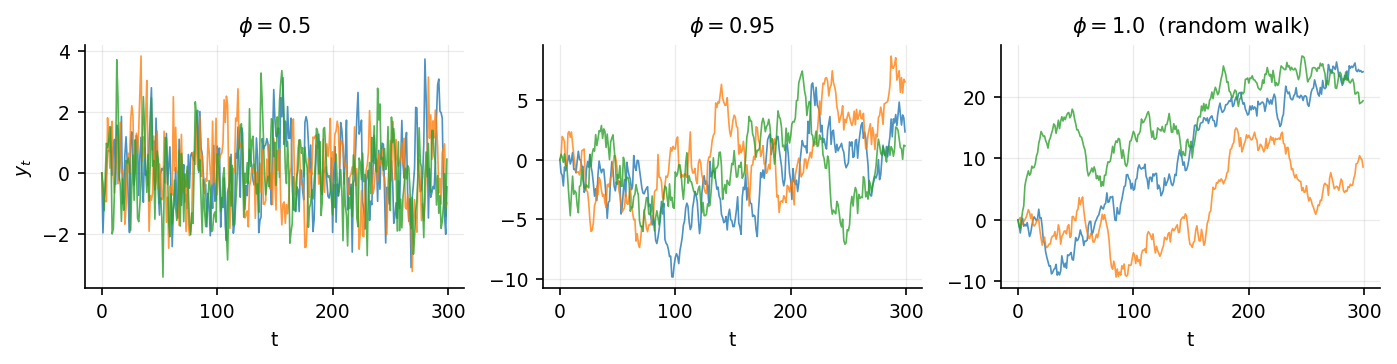
\includegraphics[width=0.94\textwidth,height=0.4\textheight,keepaspectratio]{cha11_ar1_paths.png}
  \end{center}
  \begin{takeaway}[{{The knife edge at $\phi = 1$}}]
    \footnotesize
    For $|\phi| < 1$ the series forgets: shocks decay like $\phi^k$, the mean
    $\beta_0/(1-\phi)$ exists, forecasts converge to it. At $\phi = 1$ --- the
    \textbf{random walk} --- shocks never decay, the variance grows without bound,
    and the best forecast of every horizon is \emph{today's value}. Financial
    prices live at this edge; that is the postscript.
  \end{takeaway}
\end{frame}

\begin{frame}{Exercise A11.3 --- AR(1) arithmetic [Math]}
  \begin{exercise}
    A stationary AR(1): $y_t = 2 + 0.8\, y_{t-1} + \varepsilon_t$, and today
    $y_T = 14$.
    \begin{enumerate}
      \item Compute the long-run mean of the process.
      \item Compute the one- and two-step forecasts
            $\hat y_{T+1\mid T}$ and $\hat y_{T+2\mid T}$.
      \item Where do the forecasts head as the horizon grows, and why is that the
            honest answer?
    \end{enumerate}
  \end{exercise}
\end{frame}

\begin{frame}{Solution --- Exercise A11.3}
  \begin{solutionbox}
    \footnotesize
    \textbf{Part 1.} Take expectations of both sides at stationarity,
    $\mu = 2 + 0.8\mu$, so $\mu = 2/(1 - 0.8) = \mathbf{10}$.
    \par\smallskip
    \textbf{Part 2.} Set future noise to its mean (zero):
    $\hat y_{T+1\mid T} = 2 + 0.8 \times 14 = \mathbf{13.2}$;
    $\hat y_{T+2\mid T} = 2 + 0.8 \times 13.2 = \mathbf{12.56}$.
    \par\smallskip
    \textbf{Part 3.} Each step multiplies the distance from $\mu$ by $0.8$:
    $14 \to 13.2 \to 12.56 \to \dots \to 10$. The forecast decays geometrically to
    the mean because the model's memory does --- beyond its memory horizon the
    honest forecast \emph{is} the mean, with widening uncertainty. A forecast that
    stays interesting at every horizon is advertising, not statistics.
  \end{solutionbox}
  \begin{mistake}
    Forecasting $y_{T+2}$ by plugging in the \emph{observed} $y_{T+1}$ --- it does
    not exist yet. Multi-step forecasts feed the model its \emph{own} predictions,
    which is exactly why errors compound with horizon.
  \end{mistake}
\end{frame}

\begin{frame}{Forecasting the held-out week}
  \begin{center}
    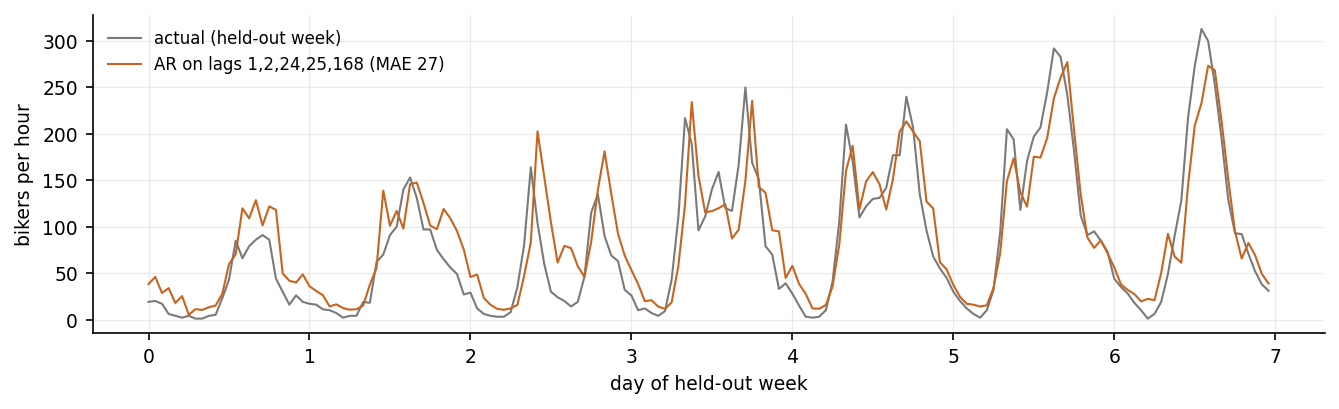
\includegraphics[width=0.9\textwidth,height=0.38\textheight,keepaspectratio]{cha11_ar.png}
  \end{center}
  \begin{numexample}[Beat the baselines or go home]
    \footnotesize
    Final week held out, model fitted strictly on the past. MAE per hour:
    global mean $\mathbf{90.5}$, seasonal naive (same hour last week)
    $\mathbf{32.7}$, our AR on lags $(1,2,24,25,168)$: $\mathbf{27.0}$.
  \end{numexample}
  \begin{takeaway}[The seasonal naive is the baseline that matters]
    \footnotesize
    Copying last week already crushes the mean. Any model you propose must beat
    \emph{that} --- many published forecasts do not.
  \end{takeaway}
\end{frame}

% ============================================================
\section{Honest Evaluation}
% ============================================================

\begin{frame}{Rolling-origin backtesting --- Chapter 5, made time-safe}
  \begin{center}
  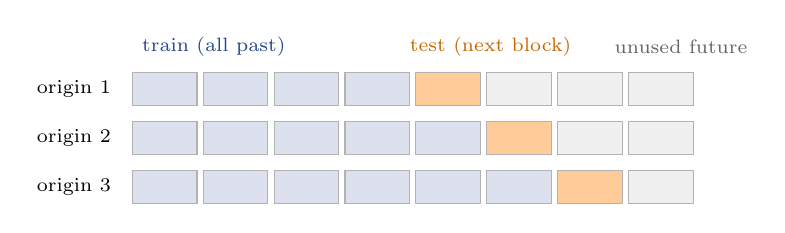
\begin{tikzpicture}[font=\scriptsize]
    \foreach \i in {0,1,2} {
      \foreach \j in {0,...,7} {
        \pgfmathtruncatemacro{\trainend}{4+\i}
        \ifnum\j<\trainend
          \fill[accent!16] (\j*0.9, -\i*0.62) rectangle ++(0.82, 0.42);
        \else
          \ifnum\j=\trainend
            \fill[orange!40] (\j*0.9, -\i*0.62) rectangle ++(0.82, 0.42);
          \else
            \fill[black!6] (\j*0.9, -\i*0.62) rectangle ++(0.82, 0.42);
          \fi
        \fi
        \draw[black!30] (\j*0.9, -\i*0.62) rectangle ++(0.82, 0.42);
      }
      \pgfmathtruncatemacro{\orig}{\i+1}
      \node[anchor=east] at (-0.15, -\i*0.62+0.21) {origin \orig};
    }
    \node[anchor=west, accent] at (0, 0.75) {train (all past)};
    \node[anchor=west, orange!80!black] at (3.4, 0.75) {test (next block)};
    \node[anchor=west, black!60] at (6.0, 0.75) {unused future};
  \end{tikzpicture}
  \end{center}
  \begin{block}{Algorithm (rolling origin)}
    \footnotesize
    For each origin $T_1 < T_2 < \dots$: fit on data up to $T_i$, forecast the next
    block, record the error; report the average. Every fold trains on the past and
    tests on the future --- deployment, rehearsed.
  \end{block}
  \begin{takeaway}[This answers Chapter 5's open question]
    Chapter 5's pitfalls slide asked how to cross-validate a time series. This is
    the answer: the folds \emph{roll forward}; they are never shuffled.
  \end{takeaway}
\end{frame}

\begin{frame}{The leak, measured}
  \begin{center}
    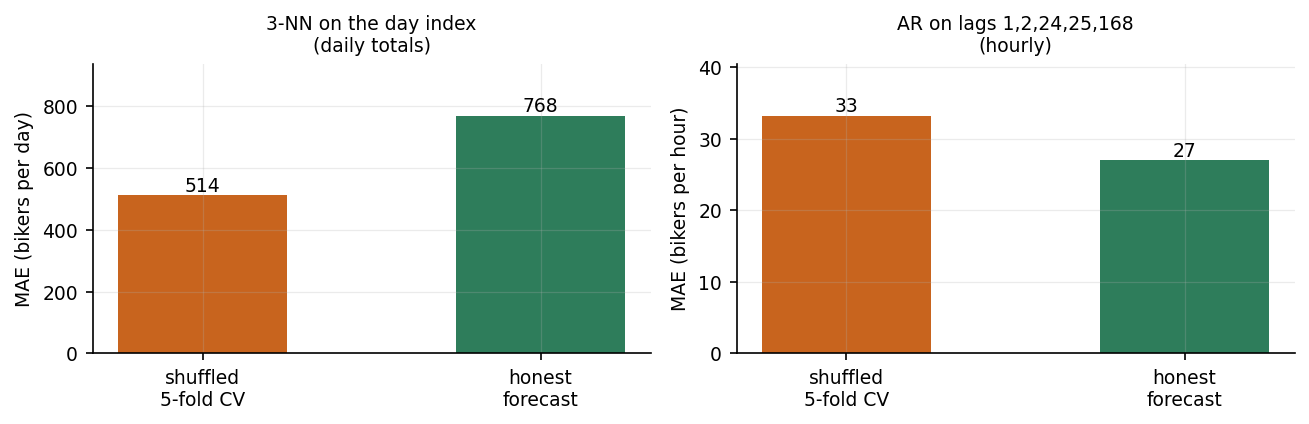
\includegraphics[width=0.86\textwidth,height=0.44\textheight,keepaspectratio]{cha11_backtest.png}
  \end{center}
  \begin{takeaway}[Shuffled CV answers a different question]
    \footnotesize
    Left, a 3-NN on the day index (daily totals): shuffled CV says
    $\mathbf{514}$; honestly forecasting the final 60 days costs $\mathbf{768}$ ---
    the CV number flatters by a third, because shuffled folds let the model
    interpolate between neighbouring days. Right, the AR on lags: $33.1$ vs
    $27.0$ --- with honest lag features the two nearly agree, and CV even errs
    \emph{pessimistic}. The gap is not a fixed tax; it depends on what the model
    can reach --- so you cannot correct for it, only avoid it.
  \end{takeaway}
\end{frame}

\begin{frame}{Exercise A11.4 --- The seasonal naive as a null model [Concept]}
  \begin{exercise}
    Your team's gradient-boosted demand model reports backtested MAE $= 31$; the
    deck omits baselines.
    \begin{enumerate}
      \item Define the two baselines you would demand, and what each one costs to
            run.
      \item On Bikeshare's held-out week those baselines score $90.5$ and $32.7$.
            Rewrite the team's headline honestly given their $31$.
      \item Name the Chapter 2 concept that explains why the naive baselines are
            so strong here.
    \end{enumerate}
  \end{exercise}
\end{frame}

\begin{frame}{Solution --- Exercise A11.4}
  \begin{solutionbox}
    \footnotesize
    \textbf{Part 1.} The \emph{global mean} (one number; free) and the
    \emph{seasonal naive} $\hat y_{t} = y_{t - s}$ (copy the last cycle; also
    free). Both need zero fitting and one line of code.
    \par\smallskip
    \textbf{Part 2.} ``Our model improves on copying last week by $1.7$ MAE points
    ($32.7 \to 31$, about $5\%$) --- and on the unconditional mean by $66\%$.''
    The second number sounds impressive and is nearly all seasonality; the first
    is the model's actual contribution.
    \par\smallskip
    \textbf{Part 3.} The bias--variance decomposition's \emph{irreducible-error}
    lesson, in time-series clothing: most of the predictable variance lives in the
    seasonal cycle, which the naive already captures at zero variance cost. The
    model competes only for the remainder.
  \end{solutionbox}
  \begin{mistake}
    Reporting improvement over the \emph{mean} when a seasonal naive exists. On
    strongly seasonal data that comparison flatters any model, including broken
    ones.
  \end{mistake}
\end{frame}

\begin{frame}{Extended Exercise A11.1 --- Build the forecaster [Python]}
  \begin{longexercise}
    Reproduce the module's forecaster from scratch on \texttt{Bikeshare.csv}:
    \begin{enumerate}
      \item Build lagged columns $(1, 2, 24, 25, 168)$ of \texttt{bikers}; hold out
            the final $168$ hours; fit OLS on the rest.
      \item Compute held-out MAE for your model, the seasonal naive
            ($y_{t-168}$) and the global mean. Target: $\approx 27$ / $32.7$ /
            $90.5$.
      \item Add the hour-of-day as $23$ dummy variables (Chapter 3 machinery) to
            the lag design. Does it help on top of the lags? Why is the answer
            close to no?
      \item Refit dropping lag $168$. Which baseline does your model now barely
            beat, and what does that teach about feature choice?
    \end{enumerate}
  \end{longexercise}
\end{frame}

\begin{frame}[fragile]{Solution --- Extended Exercise A11.1 (1/2)}
  \begin{solutionbox}[Solution --- code]
\begin{lstlisting}
import numpy as np, pandas as pd
bike = pd.read_csv("Bikeshare.csv", index_col=0)
y = bike["bikers"].to_numpy(float)
lags = [1, 2, 24, 25, 168]; p = max(lags)
X = np.column_stack([y[p-k : len(y)-k] for k in lags])
yy = y[p:]
cut = len(yy) - 168                       # final week held out
Xtr = np.column_stack([np.ones(cut), X[:cut]])
beta = np.linalg.lstsq(Xtr, yy[:cut], rcond=None)[0]
pred = np.column_stack([np.ones(168), X[cut:]]) @ beta
mae   = np.abs(yy[cut:] - pred).mean()                 # ~27.0
naive = np.abs(yy[cut:] - yy[cut-168:cut]).mean()      # ~32.7
mean_ = np.abs(yy[cut:] - yy[:cut].mean()).mean()      # ~90.5
print(f"AR {mae:.1f} | naive {naive:.1f} | mean {mean_:.1f}")
\end{lstlisting}
  \end{solutionbox}
\end{frame}

\begin{frame}{Solution --- Extended Exercise A11.1 (2/2)}
  \begin{solutionbox}[Solution --- parts 3 and 4]
    \footnotesize
    \textbf{Part 3.} The hour dummies add almost nothing: lags $24$, $25$ and $168$
    already \emph{carry} the daily shape, measured on the most recent cycles
    rather than averaged over the year. Calendar features and seasonal lags are
    two encodings of the same clock --- offering both mostly buys collinearity
    (Chapter 3's warning), not accuracy.
    \par\smallskip
    \textbf{Part 4.} Without lag $168$ the model loses the weekly rhythm ---
    Saturdays are forecast from Friday's shape. The MAE degrades toward the
    seasonal naive's $32.7$: the model now barely beats \emph{copying}, though it
    still crushes the mean. Feature choice in AR models \textbf{is} the modelling;
    the estimator never changed.
  \end{solutionbox}
  \begin{mistake}
    Standardising or shuffling the design matrix out of habit before the split.
    The split must come first and must be temporal --- every preprocessing
    statistic belongs to the training window (Chapter 5's leakage rule, sharpened
    by time).
  \end{mistake}
\end{frame}

% ============================================================
\section{A Financial Postscript}
% ============================================================

\begin{frame}{Why Chapter 4 could barely predict the market}
  \begin{center}
    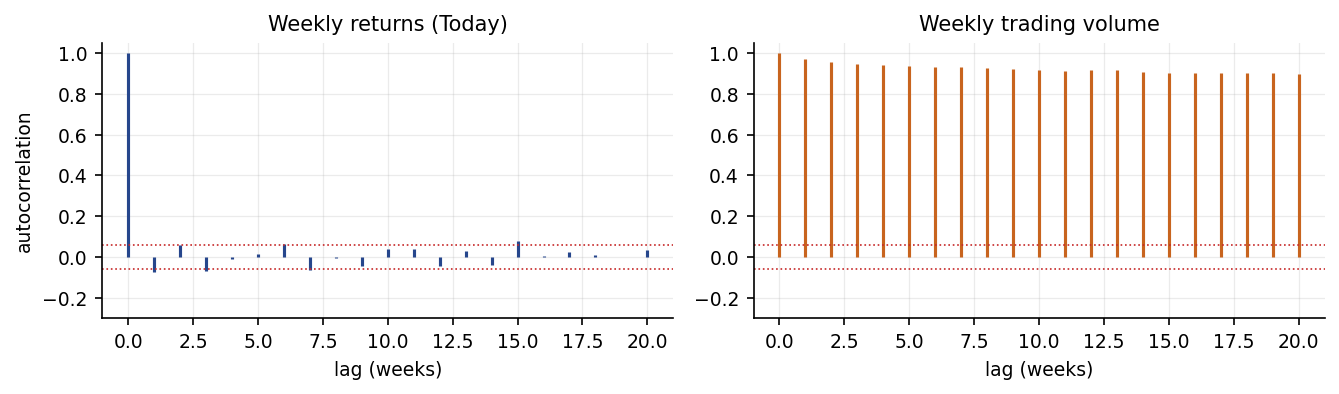
\includegraphics[width=0.94\textwidth,height=0.42\textheight,keepaspectratio]{cha11_weekly_acf.png}
  \end{center}
  \begin{takeaway}[{{Two series from the same file, two different worlds}}]
    \footnotesize
    \texttt{Weekly} returns: $r_1 = -0.075$, inside the $\pm 0.059$ band almost
    everywhere --- close to white noise, which is \emph{why} Chapter 4's classifiers
    hovered at chance. Trading \emph{volume}: $r_1 = 0.973$, extremely forecastable.
    Efficient markets erase autocorrelation in \textbf{returns} (any pattern would
    be traded away), but not in activity.
  \end{takeaway}
\end{frame}

\begin{frame}{Exercise A11.5 --- Reading the two ACFs [Concept]}
  \begin{exercise}
    Using the previous slide's plots:
    \begin{enumerate}
      \item A consultant proposes an AR(5) on \texttt{Weekly} returns to time the
            market. Expected out-of-sample $R^2$, roughly --- and why?
      \item The same consultant proposes an AR model for next week's trading
            \emph{volume}. Reasonable?
      \item Connect this to the random-walk panel of the stationarity slide: which
            object in finance is (approximately) the random walk --- prices,
            returns, or volume?
    \end{enumerate}
  \end{exercise}
\end{frame}

\begin{frame}{Solution --- Exercise A11.5}
  \begin{solutionbox}
    \footnotesize
    \textbf{Part 1.} Roughly zero. The lag-1 autocorrelation of $-0.075$ caps the
    linear predictability: an AR(1) explains about $r_1^2 \approx 0.6\%$ of the
    variance in-sample, and even that mostly evaporates out of sample. This is the
    same wall \texttt{Smarket} hit in Chapter 4 --- it is a property of the data,
    not of the model.
    \par\smallskip
    \textbf{Part 2.} Yes --- $r_1 = 0.973$ means volume is highly persistent;
    a small AR fits it well. Not everything financial is unforecastable: only the
    part whose forecastability someone could monetise.
    \par\smallskip
    \textbf{Part 3.} \emph{Prices}: if returns (the differences) are white noise,
    the price level is their running sum --- a random walk, the $\phi = 1$ panel.
    Differencing a random walk yields the stationary object; that is why one
    models returns, never price levels.
  \end{solutionbox}
  \begin{mistake}
    Fitting on price \emph{levels} and celebrating $R^2 = 0.99$. A random walk
    regressed on its own lag always yields $R^2 \approx 1$ and forecasts nothing;
    the information is in the differences.
  \end{mistake}
\end{frame}

\begin{frame}{Extended Exercise A11.2 --- Design the backtest [Integrative]}
  \begin{longexercise}
    A retailer wants daily demand forecasts, horizon $14$ days, for $200$ stores;
    promotions are known in advance; the assortment changed structurally $10$
    months ago. Design the evaluation:
    \begin{enumerate}
      \item Specify the backtest: window type (expanding or sliding), origin
            spacing, horizon, and metric --- with one sentence of justification
            each.
      \item Which two baselines go in every report?
      \item The structural break: how does it change your training window, and
            what does it do to the stationarity assumption?
      \item A colleague proposes tuning hyperparameters with shuffled CV
            \emph{inside} each training window, keeping the outer backtest
            temporal. Legitimate or leak?
    \end{enumerate}
  \end{longexercise}
\end{frame}

\begin{frame}{Solution --- Extended Exercise A11.2}
  \begin{solutionbox}
    \footnotesize
    \textbf{Part 1.} \emph{Sliding} window (the break makes ancient data
    misleading); origins every $7$ days (dense enough to average over weekday
    effects, cheap enough to run); horizon exactly $14$ days ahead (evaluate what
    you will deploy); MAE per store-day, aggregated per horizon step (day-1 and
    day-14 accuracy differ and both matter).
    \par\smallskip
    \textbf{Part 2.} Global (or per-store) mean, and the seasonal naive
    $y_{t-7}$. Improvements are quoted against the naive.
    \par\smallskip
    \textbf{Part 3.} Either start training after the break or down-weight the old
    regime; stationarity holds at best \emph{within} regimes. Ten months of daily
    data per store is workable. The backtest must also not average across the
    break, or it scores a regime nobody will face again.
    \par\smallskip
    \textbf{Part 4.} Legitimate as a pragmatic approximation --- the future
    relative to each \emph{outer} test block is untouched, so the reported number
    stays honest. But the tuned hyperparameters may still favour interpolators
    (part 3 of the leak story), so temporal inner folds are the safer default.
  \end{solutionbox}
\end{frame}

% ============================================================
\section{Python Lab}
% ============================================================

\begin{frame}{Python lab --- run it live}
  \begin{labnote}[{{Reproduce every number: \texttt{make\_figures.py}}}]
    Every number on these slides is computed by \texttt{make\_figures.py} in this
    module's folder, from the bundled \texttt{Bikeshare.csv} and
    \texttt{Weekly.csv} --- run it and read it alongside the deck:
    \begin{itemize}
      \item the from-scratch ACF ($r_1 = 0.84$, $r_{24} = 0.79$, band $\pm 0.021$);
      \item the AR-on-lags forecaster and its baselines ($27.0$ / $32.7$ / $90.5$);
      \item the leak experiment: shuffled CV $514$ vs honest $768$ on daily totals;
      \item the \texttt{Weekly} postscript ($r_1 = -0.075$ returns, $0.973$ volume).
    \end{itemize}
    A companion notebook in the course lab format is in preparation; until it
    lands, the script \emph{is} the lab --- it runs top to bottom in the course
    environment with no extra packages.
  \end{labnote}
\end{frame}

\begin{frame}[fragile]{The whole module in fourteen lines}
\begin{lstlisting}
import numpy as np, pandas as pd
bike = pd.read_csv("Bikeshare.csv", index_col=0)
y = bike["bikers"].to_numpy(float)

def acf(x, k):                       # correlation with your own past
    d = x - x.mean()
    return (d[k:] * d[:-k]).sum() / (d * d).sum()
print(f"r1 = {acf(y,1):.2f}, r24 = {acf(y,24):.2f}")   # 0.84, 0.79

lags = [1, 2, 24, 25, 168]; p = max(lags)              # AR = Ch.3 on lags
X = np.column_stack([np.ones(len(y)-p)]
                    + [y[p-k:len(y)-k] for k in lags])
beta = np.linalg.lstsq(X[:-168], y[p:-168], rcond=None)[0]
mae = np.abs(y[-168:] - X[-168:] @ beta).mean()
print(f"held-out week MAE = {mae:.1f}")                # 27.0
\end{lstlisting}
\end{frame}

% ============================================================
\section{Summary}
% ============================================================

\begin{frame}{Module A11 in one slide}
  \begin{block}{What we accomplished}
    Took the course's machinery to ordered data --- and replaced the one habit
    (shuffling) that ordered data forbid.
  \end{block}
  \begin{itemize}
    \item The order is the information: Bikeshare's daily and weekly clocks
          dominate everything.
    \item The ACF measures memory: $r_1 = 0.84$, $r_{24} = 0.79$ against a
          $\pm 0.021$ noise band --- computed by hand and in code.
    \item AR($p$) is least squares on lagged copies; stationarity ($|\phi| < 1$)
          is what makes it meaningful.
    \item Baselines first: mean $90.5$, seasonal naive $32.7$, our AR $27.0$
          MAE on a truly held-out week.
    \item Evaluation must roll forward: shuffled CV said $514$ where reality said
          $768$ on daily totals.
    \item Financial returns are the null case: $r_1 = -0.075$ --- nothing to
          forecast, by design of the market.
  \end{itemize}
\end{frame}

\begin{frame}{Key formulas at a glance}
  \footnotesize
  \begin{description}
    \item[ACF] $r_k = \sum_{t>k} (y_t - \bar y)(y_{t-k} - \bar y) \big/
      \sum_t (y_t - \bar y)^2$; noise band $\pm 1.96/\sqrt{T}$.
    \item[AR($p$)] $y_t = \beta_0 + \sum_{j} \phi_j\, y_{t-k_j} + \varepsilon_t$,
      fitted by OLS on lagged columns.
    \item[AR(1) mean] $\mu = \beta_0 / (1 - \phi)$, provided $|\phi| < 1$.
    \item[AR(1) forecast] $\hat y_{T+h\mid T} = \mu + \phi^h (y_T - \mu)$ ---
      geometric decay to the mean.
    \item[Seasonal naive] $\hat y_t = y_{t-s}$ (here $s = 168$ hours).
    \item[Random walk] $\phi = 1$: forecast $=$ today, variance grows with $h$;
      difference it to get stationarity.
  \end{description}
\end{frame}

\begin{frame}{Vocabulary checklist}
  \footnotesize
  \begin{center}
  \begin{tabular}{@{}ll@{}}
    \toprule
    \textbf{Term} & \textbf{Meaning} \\
    \midrule
    lag & the series shifted back $k$ steps \\
    autocorrelation (ACF) & correlation between $y_t$ and $y_{t-k}$ \\
    white noise & no autocorrelation at any lag; unforecastable \\
    stationarity & distribution of $(y_t, y_{t+k})$ free of $t$ \\
    AR($p$) & regression of $y_t$ on its last $p$ values \\
    random walk & AR(1) with $\phi = 1$; difference before modelling \\
    seasonal naive & forecast by copying the last full cycle \\
    horizon & how far ahead a forecast reaches \\
    rolling-origin backtest & train on past, test on next block, roll forward \\
    leakage (temporal) & any future information touching the training side \\
    \bottomrule
  \end{tabular}
  \end{center}
\end{frame}

\begin{frame}{Decision rules of thumb}
  \begin{itemize}
    \item Plot the series in order before anything else; then plot the ACF.
    \item ACF flat inside $\pm 1.96/\sqrt{T}$ $\Rightarrow$ stop --- report the
          mean and its uncertainty; there is nothing to model.
    \item Offer the model the lags the ACF points at (recent, one cycle back, one
          long cycle back) --- not every lag up to $200$.
    \item Trend or unit root in sight $\Rightarrow$ difference first (returns, not
          prices).
    \item Always run the two free baselines; quote your gain against the
          \emph{seasonal naive}.
    \item Evaluate with a rolling origin at the deployment horizon. Never shuffle.
    \item Preprocessing statistics (means, scalers) come from the training window
          only.
  \end{itemize}
\end{frame}

\begin{frame}{Common pitfalls}
  \begin{alertblock}{Don't}
    \begin{enumerate}
      \item Shuffle time-ordered rows into CV folds and call the score honest.
      \item Report improvement over the global mean when a seasonal naive exists.
      \item Fit levels of a random walk and admire the $R^2$.
      \item Feed multi-step forecasts observed future values instead of their own
            predictions.
      \item Fit one model across a structural break as if the regime never
            changed.
      \item Read a long-horizon forecast that never widens as anything but
            overconfidence.
    \end{enumerate}
  \end{alertblock}
\end{frame}

\begin{frame}{Self-check questions}
  \scriptsize
  \begin{readme}[{{Quick self-assessment}}]
    \begin{enumerate}
      \item For $y = (3,5,4,6,5,7)$: $r_1$ and $r_2$?
      \item An AR(1) has $\beta_0 = 2$, $\phi = 0.8$, $y_T = 14$. Long-run mean and
            the next two forecasts?
      \item Bikeshare's held-out-week MAEs were $90.5$ / $32.7$ / $27.0$. Which
            estimator is which, and which comparison should a report headline?
      \item Why did shuffled CV report $514$ where the honest forecast cost $768$
            --- and why did the same comparison for the AR model nearly agree?
      \item \texttt{Weekly} returns have $r_1 = -0.075$ with band $\pm 0.059$.
            What follows for market-timing models?
      \item What single transformation turns a random walk into something
            stationary?
    \end{enumerate}
  \end{readme}
  \begin{takeaway}[{{Answers}}]
    (1) $-0.1$ and $+0.4$. (2) $\mu = 10$; $13.2$, then $12.56$. (3) Global mean /
    seasonal naive / AR on lags; headline the gain over the \emph{naive}
    ($32.7 \to 27.0$). (4) Shuffled folds let the 3-NN interpolate between
    neighbouring days; the AR's lag features grant no such shortcut, so its two
    scores nearly coincide --- the leak's size depends on the model. (5) Linear
    predictability is capped near $r_1^2 \approx 0.6\%$ --- practically nil.
    (6) Differencing: model the changes, not the levels.
  \end{takeaway}
\end{frame}

\begin{frame}{Five things to remember}
  \begin{takeaway}[Module A11 in five lines]
    \begin{enumerate}
      \item \textbf{The order is the information} --- shuffling destroys the very
            structure you would model.
      \item \textbf{The ACF is the instrument:} $0.84$ at lag 1 and $0.79$ at lag
            24 told us which lags to offer before any model was fitted.
      \item \textbf{An AR model is Chapter 3 on lagged copies} --- the estimator is
            old; the feature choice is the craft.
      \item \textbf{Beat the seasonal naive or say so} --- $32.7 \to 27.0$ is the
            honest headline; $90.5 \to 27.0$ is mostly the clock.
      \item \textbf{Evaluate by rolling forward, never by shuffling} --- the leak
            ($514$ vs $768$) is unfixable after the fact.
    \end{enumerate}
  \end{takeaway}
\end{frame}

\begin{frame}{What's next}
  \begin{itemize}
    \item \textbf{Module A3 --- Conformal Prediction} named time order as the thing
          that breaks exchangeability; this module is what you do about it.
          Conformal variants for time series exist --- built on the rolling origins
          you now run.
    \item \textbf{Module A10 --- Causal Inference from Observational Data}:
          difference-in-differences is a time-series design at heart; parallel
          trends is a statement about two series' common structure.
    \item \textbf{Chapter 8's boosting} plus this module's lag features is the
          workhorse forecaster in industry --- the design matrix is the same one
          you built here.
  \end{itemize}
\end{frame}

% ============================================================
\appendix
\AtBeginSection[]{}
\section{Appendix: optional and advanced material}
% ============================================================

\begin{frame}{Appendix --- what is in here, and why}
  \footnotesize
  Nothing in the appendix is needed to follow the module: each slide is a formal
  derivation, a longer worked exercise, or a side topic. Read it when you want the
  full story, or when a later chapter sends you back here.
  \begin{block}{Contents of the appendix}
    \begin{itemize}
      \item \textbf{AR(1) mean and variance, derived} --- two lines each; moved out
            because the results, not the algebra, carry the main deck.
      \item \textbf{From AR to ARMA and friends} --- a map of the classical model
            zoo and what each letter buys; look-up material, not narrative.
      \item \textbf{Forecast intervals} --- why uncertainty must widen with the
            horizon, and the AR(1) formula that widens it.
    \end{itemize}
  \end{block}
\end{frame}

\begin{frame}{AR(1) moments, derived}
  \footnotesize
  Stationary AR(1): $y_t = \beta_0 + \phi y_{t-1} + \varepsilon_t$,
  $\operatorname{Var}(\varepsilon_t) = \sigma^2$, $|\phi| < 1$.
  \begin{block}{Mean}
    Expectations of both sides: $\mu = \beta_0 + \phi\mu \Rightarrow
    \mu = \beta_0/(1-\phi)$.
  \end{block}
  \begin{block}{Variance and ACF}
    Variances of both sides (independence of $\varepsilon_t$ from the past):
    $v = \phi^2 v + \sigma^2 \Rightarrow v = \sigma^2/(1-\phi^2)$. Multiplying the
    defining equation by $y_{t-k}$ and taking expectations gives
    $\rho_k = \phi^k$ --- geometric decay, the signature shape.
  \end{block}
  \begin{takeaway}[{{Why $\phi = 1$ destroys everything}}]
    Both denominators hit zero: no stationary mean, no stationary variance. Every
    formula on the main deck quietly assumed $|\phi| < 1$; this is where.
  \end{takeaway}
\end{frame}

\begin{frame}{The classical zoo, in one table}
  \footnotesize
  \begin{center}
  \begin{tabular}{@{}lll@{}}
    \toprule
    \textbf{Model} & \textbf{Adds} & \textbf{Use when} \\
    \midrule
    MA($q$) & lagged \emph{errors} as predictors & short, sharp memory \\
    ARMA($p,q$) & both memories & parsimony over a long AR \\
    ARIMA($p,d,q$) & $d$ rounds of differencing & trends / unit roots \\
    SARIMA & seasonal AR/MA terms at lag $s$ & one dominant seasonal cycle \\
    ETS & explicit trend + seasonal components & business series, automatic use \\
    \bottomrule
  \end{tabular}
  \end{center}
  \begin{readme}[How to place this module in the zoo]
    Our lag-selected AR with seasonal lags ($24$, $168$) is a hand-built cousin of
    SARIMA --- same idea, plain OLS. \texttt{statsmodels.tsa} fits the full zoo;
    the diagnostics (ACF, baselines, rolling origin) transfer unchanged, and they
    are the part that decides whether \emph{any} member of the zoo is working.
  \end{readme}
\end{frame}

\begin{frame}{Forecast intervals widen --- by law, not by taste}
  \footnotesize
  For a stationary AR(1), the $h$-step forecast error is
  $\sum_{j=0}^{h-1} \phi^j \varepsilon_{T+h-j}$, so
  \[
    \operatorname{Var}\big(y_{T+h} - \hat y_{T+h\mid T}\big)
      = \sigma^2 \sum_{j=0}^{h-1} \phi^{2j}
      = \sigma^2\,\frac{1 - \phi^{2h}}{1 - \phi^2}
      \;\xrightarrow[h \to \infty]{}\; \frac{\sigma^2}{1 - \phi^2}
      = \operatorname{Var}(y).
  \]
  \begin{takeaway}[The honest endpoint]
    As the horizon outruns the memory, the forecast variance climbs to the
    series' \emph{own} variance: at long horizons you know nothing beyond the
    unconditional distribution --- which is exactly what the point forecast
    (decay to $\mu$) was already admitting. Module A3's conformal machinery can
    calibrate these intervals empirically from rolling-origin errors.
  \end{takeaway}
\end{frame}

\end{document}
